\chapter{Datenverarbeitung}

Wie bei jeder Anwendung von maschinellen Lernverfahren sind die zugrundeliegenden Daten von äußerster Wichtigkeit.
Im Rahmen dieser Masterarbeit wurden zweierlei Sorten von Daten benutzt:
Einmal wurden am \textit{TableSort} Schüttgutsortierer des Fraunhofer IOSBs Aufnahmen gemacht, 
die dann über mehrere Arbeitsschritte in das richtige Datenformat übersetzt wurden.
Zudem existieren simulierte Datensatze, die mit der \textit{Diskrete-Elemente-Methode} (DEM) simuliert wurden. 



\section{Datenformatierung}

\color{blue}
\begin{itemize}
	\item Zu Beginn des Datenverarbeitungskapitel erstmal definieren wie unsere Feature-Label Paare aussehen.
	\item Features eigentlich immer gleich:
	\item die Positionen der letzten \(n\) Zeitschritte (FeatureSize Hyperparameter)
	\item also ein \(2n\) Tupel, mit jeweils \(n\) X-Koordinaten und \(n\) Y-Koordinaten
	% \item \(n\) \textit{n} \(n\) \(n\) \textit{n}
\end{itemize}

Labels: Unterscheidung nach Anwendung:

NextStep: Label ist 2-Tupel, X und Y Koordinate
Separator: 
	gegeben ist eine Stelle entlang der Bewegungsrichtung der Teilchen an der der Separator angebracht ist.
	erstes element des Label ist die Koordinate entlang der orthogonalen Achse zur Bewegungsrichtung wo das Teilchen den Separator passiert
	zweites Element ist die Anzahl von Zeitschritten , die das Teilchen noch bis zum Separator braucht.

Important Point: Labels wurden normalisiert und Standardisiert ( \(\frac{TrueVal - Mean}{Standard Diviation}\))
um auszugleichen, dass sich Position und Zeitschritte auf unterschiedlichen Skalen bewegen und dementsprechend unterschiedlich hohe gradienten haben.


Es ist implementiert, dass die verschiedenen Dimensionen unterschiedlich stark gewichtet werden können - Je nach Schüttgut/präzision des Separators
Aber für die evaluierung ist keine Gewichtung vorgenommen worden.

optional: Histogramme über die Daten (mehr Teilchen in der Mitte bei Location...)
\color{black}

Welches Format die Daten annehmen unterscheidet sich leicht zwischen den beiden Anwendungen.
Die Feature-Label Paare der unterschiedlichen Anwendungen unterscheiden sich nur in den Labeln.
Die Eingangsdaten sind -- abhängig von einem Hyperparameter --
in beiden Fällen die Position des Partikels zu den letzten \(n\) Zeitschritten.
Deshalb muss kein Unterschied bezüglich der gespeicherten Tracks gemacht werden.

Dieser Hyperparameter wird \textit{FeatureSize} genannt. 
Die Features sind also ein \(2n\)-Tupel, bestehend aus \(n\) X-Koordinaten und \(n\) Y-Koordinaten.
Was die Reihenfolge angeht, so ist sie für das neuronale Netz egal, solange sie konsistent zwischen Training und Evaluation bleibt.

In der umgesetzten Implementierung ist es so, dass zuerst die X-Koordinaten 
und dann die Y-Koordinaten in chronologischer Reihenfolge aufgereiht sind. 



Die Labels, die das NextStep-Netz benutzt, sind \(2\)-Tupel.
Es handelt sich um die nächste Zeile in der Doppelspalte des dazugehörigen Tracks:
Das erste Element ist die X-Koordinate der Position des Partikels im nächsten Zeitschritt und das Zweite ist die Y-Koordinate.

Die Labels des Separator-Netzes sind ebenfalls \(2\)-Tupel.
Im Gegensatz zu denen des NextStep-Netzes können diese nicht direkt aus der CSV-Datei ausgelesen werden, sondern müssen berechnet werden.
Dies ist in Abbildung~\ref{fig:Schnittpunkt} dargestellt.
Für jedes Partikel \(i\) müssen die Positionen \(f_n\) und \(f_{n+1}\) direkt vor 
und direkt nach der Position des Druckluftdüsenarrays bestimmt werden.

Das erste Element eines Labels ist die Koordinate entlang der Achse orthogonal zur Bewegungsrichtung des Förderbandes, wo das Teilchen den Druckluftdüsenarrays passiert.
Diese erhalten wir in dem wir den Schnittpunkt zwischen der Strecke, die \(f_n\) und \(f_{n+1}\) verbindet und 
einer gedachten Gerade orthogonal zur Bewegungsrichtung des Förderbandes bestimmen.
Das zweite Element ist die Zeit, die das Partikel noch brauchen wird, bis es das Druckluftdüsenarray passiert.
Sie wird in der Einheit Frames angegeben.
Die ganzzahlige Komponente hiervon ist durch das Zählen von Elementen im Track zu bestimmen.
Die Nachkommastelle wird bestimmt als das Verhältnis von der Distanz zwischen \(f_n\) und \(s\), 
und der Distanz zwischen \(f_n\) und \(f_{n+1}\).
Dabei wird die angenommen, dass die Geschwindigkeit des Partikels zwischen \(f_n\) und \(f_{n+1}\) konstant ist.
Dies ist zwar nur eine Approximation, diese ist jedoch ausreichend gut und wird auch in~\cite{Pfaff2018} getroffen wurde.
\todo[inline]{Example: Gegeben ein Track, was für Features und Labels würden da rausfallen}


Um zu verhindern, dass verschiedene Dimensionen basierend auf ihrer Skalierung beim Gradientenabstieg unterschiedlich 
stark gewichtet werden, werden die Labels folgendermaßen standardisiert.
Jedes Element \(e\) vom Typ 1 oder Typ 2 wird entsprechend seiner Spalte behandelt, vor dem Training angepasst

\begin{equation*}
	e_{\text{neu}} = \frac{e - \mu_{\text{Typ}}}{\sigma_{\text{Typ}}}
\end{equation*}

und Ausgaben des Netzes müssen umkehrt zurück in die ursprünglichen Skalierung gerechnet werden.
\todo{überlegen wie ich klar mache, dass es sich um den durchschnitt und die Abweichung der jeweiligen Spalte handelt}

Solch ein Ungleichgewicht würde zum Beispiel auftreten, wenn sich die Werte des einen Elements im Bereich zwischen 0 und 1700 bewegen, während die des Anderen zwischen 1 und 25,
so wie es bei der Separator Anwendung der Fall sein kann.   
Theoretisch wäre es möglich beim NextStep Fall darauf zu verzichten, aber im Sinne der Einheitlichkeit wurde 
die Standardisierung für beide Fälle implementiert.


Im Code gibt es die Möglichkeit unterschiedliche Ausgaben unterschiedlich zu gewichten, indem weighted Mean Squared Error als Fehlerfunktion verwendet werden kann. 
Von dieser Möglichkeit wird in den später vorgestellten Ergebnissen nicht gebrauch gemacht, beziehungsweise den beiden Elementen wird jeweils das Gewicht 1.0 zugewiesen.
\todo{hier noch schreiben, warum man das tun wollen könnte, oder nicht?}

\begin{figure}[h]
	\centering
	% \missingfigure{geometrische Bestimmung des Schnittpunkts mit dem Separator}
	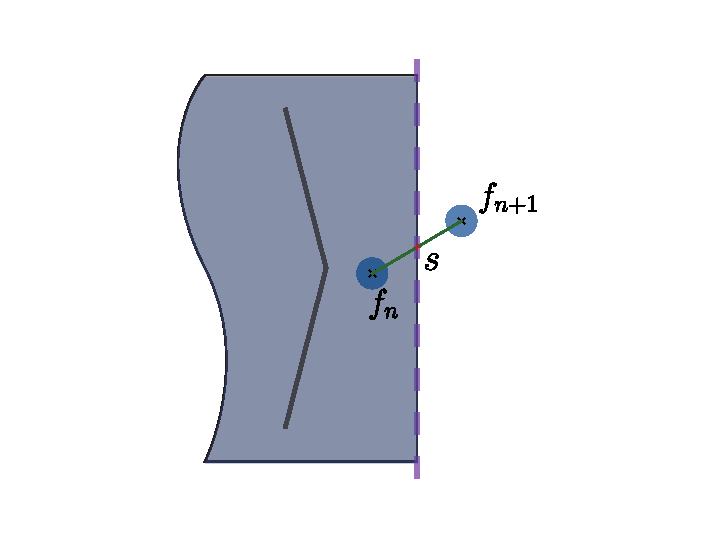
\includegraphics[width=\textwidth]{geometrie}
	\caption{Geometrische Bestimmung der Labels, nach \cite{Pfaff2018}}
	% \todo{Quelle - test?}
	\label{fig:Schnittpunkt}
\end{figure}

\section{Eigene Aufnahmen}

\subsection{Versuchsaufbau}

\color{blue}
\begin{itemize}
	\item Am TableSort System, einmal Band, einmal Rutsche
	\item Beschreibung von der Bonito Kamera, stats usw.
	\item Umrechengröße pixel zu mm
	\item Bandgeschwindigkeit
\end{itemize}
\color{black}


Zur Aufnahme der Daten wurde eine Bonito CL-400 200 FPS Kamera benutzt, die in Abbildung~\ref{pictureCam} zu sehen ist.
Die ist, wie in Abbildung~\ref{fig:tablesortsystem} oberhalb des Förderbandes angebracht.
Die Bilder, die von der Kamera aufgenommen werden, haben eine Auflösung von 2320x1726 Pixeln~\cite{alliedvisiontechnologiesgmbh2014}.
\todo[inline]{Umrechengröße pixel zu mm, im weiteren verlauf werden pixel benutzt}

\begin{figure}[h]
    \centering
    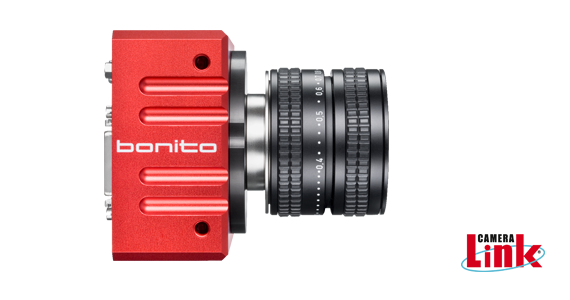
\includegraphics[width=\textwidth]{img/banner-Bonito_cropped}
    \caption{Zur Aufnahme verwendete Kamera [TODO: Quelle Bild]}
    \label{pictureCam}
\end{figure}

\subsection{Schüttgüter-Typen}

Aufgenommen wurden vier verschiedene Schüttgüter, die in Abbildung~\ref{fig:schuettgueterSchuessel} zu sehen sind, auf dem Förderband.

\begin{itemize}
    \item Kugeln
    \item grüne Pfefferkörner
    \item Zylinder
    \item Weizenkörner
\end{itemize}

Die Kugeln und der Pfeffer sowie die Zylinder und die Weizenkörner bilden jeweils 
ein Paar aus einem geometrischen Körper und einem echten Objekt, das grob dessen Form ähnelt.

Die Kugeln bestehen aus Holz und haben einen Durchmesser von 5\si{\milli\metre}.
Die Zylinder bestehen ebenfalls aus Holz. Sie haben eine Länge von 1\si{\centi\metre} und einen Durchmesser von 3\si{\milli\metre}.
Die Schüttgüter sind in Abbildung~\ref{fig:schuettgueterSchuessel} in Schüsseln 
und in Abbildung~\ref{fig:schuettgueterBand} auf dem Förderband zu sehen.
\todo{Mehr Details?}

Zusätzlich dazu wurden Kugeln und Pfefferkörner auf der Rutschenkonfiguration des \textit{TableSort} Systems aufgenommen.
\todo[inline]{Bilder einfügen}

\begin{figure}[h]
	\centering
	\begin{subfigure}[t]{0.4\textwidth}
		\centering
		\includegraphics[width=\textwidth]{kugel_001_00084_debayer}
		\caption{Kugeln auf dem Förderband}
	\end{subfigure}
	\quad
	\begin{subfigure}[t]{0.4\textwidth}
		\includegraphics[width=\textwidth]{Pfeffer_003_00020_debayer}
		\caption{Pfeffer auf dem Förderband}
	\end{subfigure}
	\vskip\baselineskip
	\begin{subfigure}[t]{0.4\textwidth}
		\includegraphics[width=\textwidth]{zylinder_001_00009_debayer}
		\caption{Zylinder auf dem Förderband}
	\end{subfigure}
	\quad
	\begin{subfigure}[t]{0.4\textwidth}
		\includegraphics[width=\textwidth]{weizen_004_00016_debayer}
		\caption{Weizen auf dem Förderband}
	\end{subfigure}
	\vskip\baselineskip
	\begin{subfigure}[t]{0.4\textwidth}
		\includegraphics[width=\textwidth]{kugeln_rutsche_013_00043_debayer}
		\caption{Kugeln auf der Rutsche}
	\end{subfigure}
	\quad
	\begin{subfigure}[t]{0.4\textwidth}
		\includegraphics[width=\textwidth]{pfeffer_rutsche_005_00056_debayer}
		\caption{Pfeffer auf der Rutsche}
	\end{subfigure}
	\caption{Verschiedene Schüttgüter auf dem Förderband bzw. der Rutsche}
	\label{fig:schuettgueterBand}
\end{figure}


\section{Datenpipeline} \label{sec:pipeline}

\color{blue}
\begin{itemize}
	\item Beschreiben wie aus den Bildern die relevanten Features extrahiert werden.
	\item Ursprungs: Bayer Matrix Bitmap
	\item Konvert to RGB
	\item Segmentierungsskript zu CSV No.1
	\item TrackSort Algorithmus zuweisung zu CSV No.2
	\item Das ist dann der finale Punkt von wo es in meinen Code geladen wird und der rest dort passiert 
\end{itemize}
\color{black}


Die Bonito Kamera nimmt Bilder in Form einer Bayer-Matrix auf, wie sie in~\ref{fig:bayerPattern} zu sehen ist.
Diese werden dann in Batches von je 3500 gesammelt und in Bitmap Dateien geschrieben.
\todo{Option Bayer-Matrix erklären}

\begin{figure}[h]
	% \missingfigure{bayer matrix}
	\centering
	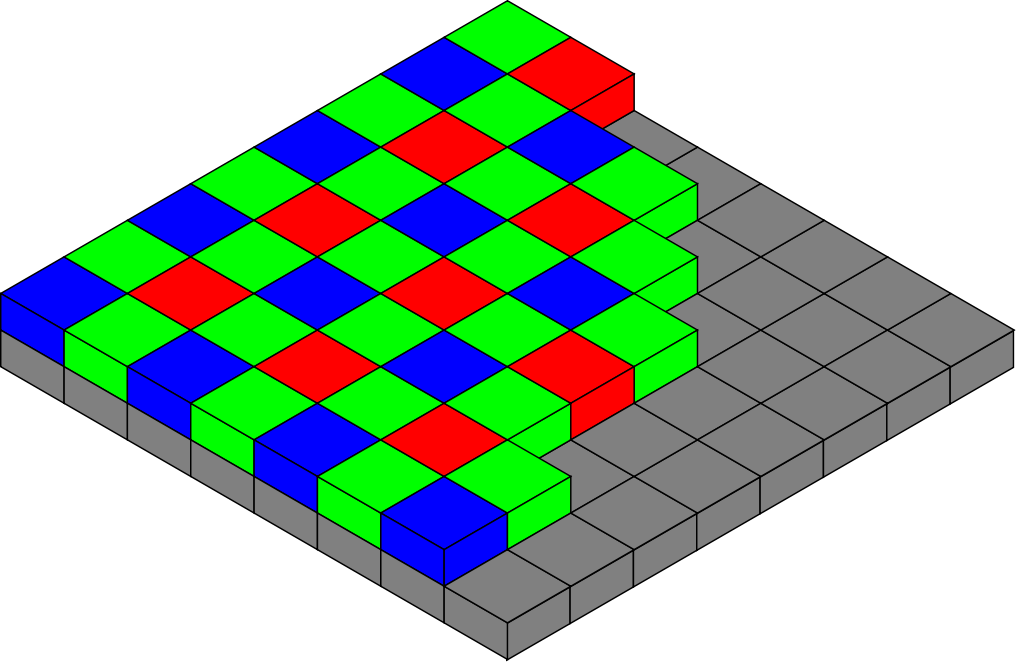
\includegraphics[width=0.6\textwidth]{1024px-Bayer_pattern_on_sensor}
	\caption{Bayer Matrix [TODO: Quelle]}
	\label{fig:bayerPattern}
\end{figure}

Auf Grund der Menge an Bildern wurden die Bilder zunächst in das PNG-Dateiformat übertragen.
Die Features, die für das Trainieren der Netze benutzt werden, sind die Koordinaten der Mittelpunkte der Objekte.
Um diese zu bestimmten, müssen zunächst die Dateien mittels \textit{demosaicing} rekonstruiert werden um gewöhnliche RGB-Bilder zu erhalten.
Die Open Source Computer Vision Library OpenCV hat eine Methode implementiert, die ein Bild von einem Farbraum in einen anderen übertragen kann.
Diese wurde eingesetzt um die einzelnen Bilder in RGB-Farbbilder zu konvertieren.
\todo[inline]{Skript ursprünglich von Georg, ein paar changes implementiert (bezüglich input und output.)}

\begin{figure}[h]
	\centering
	\begin{subfigure}[t]{0.4\textwidth}
		\includegraphics[width=\textwidth]{KugelnCropped}
		\caption{Kugeln}
	\end{subfigure}
	\quad
	\begin{subfigure}[t]{0.4\textwidth}
		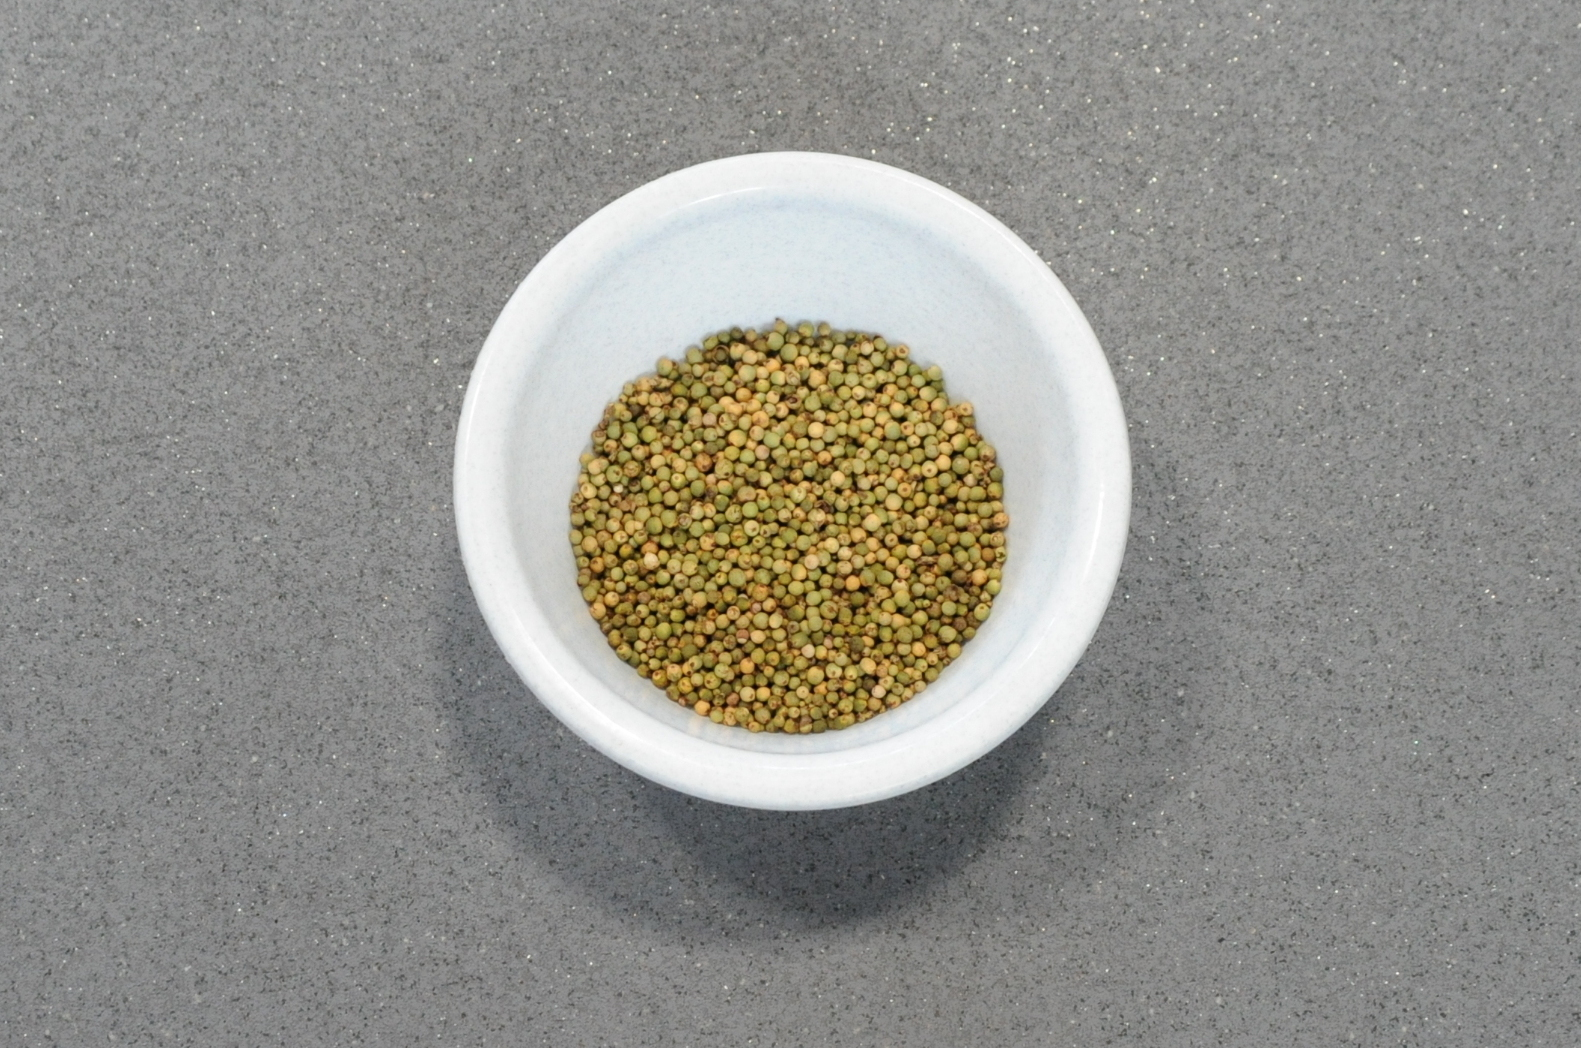
\includegraphics[width=\textwidth]{PfefferCropped}
		\caption{Pfeffer}
	\end{subfigure}
	\vskip\baselineskip
	\begin{subfigure}[t]{0.4\textwidth}
		\includegraphics[width=\textwidth]{ZylinderCropped}
		\caption{Zylinder}
	\end{subfigure}
	\quad
	\begin{subfigure}[t]{0.4\textwidth}
		\includegraphics[width=\textwidth]{WeizenCropped}
		\caption{Weizen}
	\end{subfigure}
	\caption{Verschiedene gesammelte Schüttgüter}
	\label{fig:schuettgueterSchuessel}
\end{figure}


Auf diesen kann dann eine Segmentierung vorgenommen werden.
Hierzu wurde erneut die Computer Vision Library OpenCV benutzt.
Für jede Sorte von Schüttgut wurde ein eigenes Parameterprofil von Hand angepasst.
Diese bestehen aus einem oberen und unteren Grenzwert in jedem Kanal des HSV-Raums und einer minimalen Fläche, die ein Teilchen umfassen muss.
Entsprechend der durch das Profil festgelegten Parameter werden für die einzelnen Bilder Masken angelegt,
ob die HSV-Werte der einzelnen Pixel innerhalb oder außerhalb der Grenzwerte liegen. 
Mit diesen Masken werden dann alle möglichen Konturen von Schüttgutpartikeln extrahiert, 
bevor diese noch einmal bezüglich ihrer Sinnhaftigkeit gefiltert werden. 
Im letzten Schritt wird nun der gewichtete Mittelpunkt der einzelnen Konturen bestimmt und abgespeichert.
Das Ergebnis von diesem Segmentierungsscripts ist eine CSV-Datei für jedes Batch.
Ein Beispiel für einen Ausschnitt aus solch einer Datei ist in Tabelle~\ref{table:Segmentierungsscript} zu sehen.
Eine Zeile repräsentiert jeweils ein Bild aus dem Batch, also einen Zeitschritt.
Zu Beginn jeder Zeile steht zunächst die Frame Nummer, gefolgt von der Anzahl der detektierten Partikel
und den X- und Y-Koordinaten der Mittelpunkte der detektierten Partikel.

\begin{table}[]
    \caption{Ausschnitt aus dem Ergebnis des Segmentierungsscripts}
	\small
	\centering
    \begin{tabular}{@{}rcrrrrrr@{}}
    \toprule
    Frame   & \#MP & MP\_1\_x  & MP\_1\_y  & MP\_2\_x  & MP\_2\_y  & MP\_3\_x & MP\_3\_y \\ \midrule
    636     & 1    & 1222.9975 & 92.7641   & NaN       & NaN       & NaN      & NaN      \\
    637     & 1    & 1223.4063 & 182.9758  & NaN       & NaN       & NaN      & NaN      \\
    638     & 1    & 1223.6052 & 273.2425  & NaN       & NaN       & NaN      & NaN      \\
    639     & 1    & 1223.7067 & 364.0339  & NaN       & NaN       & NaN      & NaN      \\
    640     & 1    & 1224.0704 & 453.9057  & NaN       & NaN       & NaN      & NaN      \\
    641     & 2    & 1224.2051 & 544.5191  & 1692.4549 & 43.8822   & NaN      & NaN      \\
    642     & 2    & 1224.5793 & 634.7288  & 1696.6901 & 135.9595  & NaN      & NaN      \\
    643     & 2    & 1224.9082 & 726.0094  & 1700.451  & 229.1195  & NaN      & NaN      \\
    644     & 2    & 1225.2296 & 815.9663  & 1704.1472 & 321.2075  & NaN      & NaN      \\
    645     & 2    & 1225.4286 & 906.7078  & 1708.0593 & 414.2785  & NaN      & NaN      \\
    646     & 2    & 1225.7588 & 996.0286  & 1711.5309 & 506.0545  & NaN      & NaN      \\
    647     & 3    & 1226.0411 & 1086.5729 & 1714.8831 & 599.5417  & 961.8821 & 62.7111  \\
    648     & 3    & 1226.2337 & 1175.9271 & 1718.1401 & 691.6325  & 958.5526 & 154.3124 \\
    649     & 3    & 1226.2073 & 1265.7495 & 1721.6618 & 784.5927  & 955.3107 & 246.5241 \\
    650     & 3    & 1226.2543 & 1354.9362 & 1724.9158 & 876.7192  & 952.4919 & 338.1123 \\
    651     & 3    & 1226.2634 & 1444.5903 & 1728.3341 & 970.2909  & 949.2896 & 430.9692 \\
    652     & 3    & 1226.0845 & 1533.0901 & 1732.1745 & 1062.4624 & 946.3455 & 522.8667 \\
    653     & 3    & 1225.7319 & 1621.8461 & 1735.8759 & 1155.2937 & 943.3384 & 615.4545 \\
    654     & 2    & 1739.6714 & 1247.1867 & 940.2511  & 707.7306  & NaN      & NaN      \\
    655     & 2    & 1743.4279 & 1339.4146 & 937.2216  & 800.4557  & NaN      & NaN      \\
    656     & 2    & 1747.1525 & 1430.2501 & 934.5311  & 891.7249  & NaN      & NaN      \\
    657     & 2    & 1750.9771 & 1521.8102 & 931.6626  & 984.2284  & NaN      & NaN      \\
    658     & 2    & 1754.1491 & 1612.5565 & 928.7587  & 1076.4749 & NaN      & NaN      \\
    659     & 1    & 925.8463  & 1168.794  & NaN       & NaN       & NaN      & NaN      \\
    660     & 1    & 922.8752  & 1260.7461 & NaN       & NaN       & NaN      & NaN      \\
    661     & 1    & 920.2056  & 1352.8549 & NaN       & NaN       & NaN      & NaN      \\
    662     & 1    & 917.4051  & 1444.3431 & NaN       & NaN       & NaN      & NaN      \\
    663     & 1    & 914.6493  & 1535.5131 & NaN       & NaN       & NaN      & NaN      \\
    664     & 1    & 911.8565  & 1626.5341 & NaN       & NaN       & NaN      & NaN      \\ \bottomrule
    \end{tabular}
    \normalsize
    
    \label{table:Segmentierungsscript}
    \end{table}
    

Die Mittelpunkte in dieser CSV-Datei werden nun mittels des in MATLAB implementierten \textit{Predictive Tracking} Algorithmus einzelnen Tracks zugeordnet,
\todo{Mehr details: Tracksort trackzuweisung Assignment Problem. Referenz Tobi MA?}
die dann wiederum in einer neuen CSV-Datei gespeichert werden.
Die einzelnen Tracks werden als Spaltenpaare dargestellt mit jeweils einer Spalte für die X- und Y-Koordinaten zu einem jeweiligen Zeitpunkt.
Ein Ausschnitt aus einer solchen Datei ist in Tabelle \ref{table:tracksortCSV} zu sehen.
Dies ist der Zustand in dem die Daten dann im eigentlichen Code geladen werden. 


\begin{table}[]
	\caption{Ausschnitt aus dem Ergebnis des \textit{Predictive Tracking} Algorithmus}
	\label{table:tracksortCSV}
    \small
    \centering
    \begin{tabular}{@{}rrrrrr@{}}
    \toprule
    TrackID\_4\_X & TrackID\_4\_Y & TrackID\_5\_X & TrackID\_5\_Y & TrackID\_6\_X & TrackID\_6\_Y \\ \midrule
    1036.4613     & 82.3719       & 1899.9239     & 83.2049       & 1654.4423     & 50.6811       \\
    1033.0189     & 174.9809      & 1896.8142     & 171.3283      & 1655.3193     & 143.9749      \\
    1029.6167     & 266.4979      & 1893.5937     & 259.8098      & 1656.0221     & 237.1573      \\
    1026.3908     & 358.4831      & 1890.3912     & 348.1731      & 1656.8966     & 329.8636      \\
    1023.0203     & 449.6429      & 1887.1035     & 436.4588      & 1657.6308     & 423.1592      \\
    1019.5391     & 542.2334      & 1883.7761     & 525.1073      & NaN               & NaN           \\
    NaN           & NaN           & 1880.2716     & 613.0896      & NaN           & NaN           \\
    NaN           & NaN           & 1876.6054     & 701.9719      & NaN           & NaN           \\
    NaN           & NaN           & NaN           & NaN           & NaN           & NaN           \\ \bottomrule
    \end{tabular}
\end{table}






\section{Simulierte Daten}

\color{blue}
Die DEM Daten, wo sie herkommen, was der unterschied ist zu den selbst aufgenommenen Daten. 
Vorteile und Nachteile...\cite{pieper2016numerical}, \cite{pieper2017numerical} 

Original: \SI{1000}{\hertz}, downsampled auf \SI{200}{\hertz}, 

Nicht ganz so viele Partikel, aber dafür sehr lange tracks - Informationen auf dem gesamten Band, nicht nur auf dem Part wo die Kamera drauf schaut.

Vergleich bezüglich der Eignung für die verschiedenen Ansätze dann im Evaluations Kapitel
\color{black}

Neben den selbst aufgenommenen Daten wurde im Rahmen dieser Arbeit auch mit einigen simulierten Datensätzen gearbeitet.
Diese Datensätze wurden basierend auf einer hochgenauen numerischen Simulation des \textit{TableSort} Systems mittels der Diskrete-Elemente-Methode erstellt.
[interaktion Teilchen untereinander und mit dem Sortierer]
In Abbildung~\ref{fig:DEMSimulation} ist das Modell des Schüttgutsortierers zu sehen.
Die Simulation wird mit einem Zeitschritt von \SI{1e-5}{\second} durchgeführt.
Die Positionsdaten in den Datensätzen waren ursprünglich mit einer Frequenz von \SI{1000}{\hertz} aufgelistet,
um jedoch Vergleichbarkeit mit den realen Daten zu erhalten wurde diese Frequenz auf \SI{200}{\hertz} reduziert.


Dennoch gibt es einige Unterschiede zwischen den selbst aufgenommenen Daten und denen, die simuliert wurden.
Am wichtigsten ist dabei, dass die Positionen der Simulation eine absolut verlässliche Groundtruth sind.
Das sind die Positionen der selbst aufgenommenen Daten nicht.
Während den einzelnen in Sektion~\ref{sec:pipeline} beschrieben Schritten kann es zu Fehlern kommen, die sich durch die gesamte Pipeline fortpflanzen.
Die Segmentierung kann an einigen Stellen nicht präzise sein, in dem z.\,B. ein Stück Schattens als Teil des Partikels interpretiert und dadurch den Mittelpunkt verschiebt. 
Bei einer Kollision von zwei Partikeln kann es dazu kommen, dass der \textit{Predictive Tracking} Algorithmus die beiden Tracks vertauscht.  

Desweiteren bewegt sich das Förderband in der Simulation mit \SI{1.5}{\meter\per\second}, 
während Messungen am realen \textit{TableSort} System darauf hindeuten, dass das Förderband dort nur eine Geschwindigkeit von 
circa \SI{1.1}{\meter\per\second} hat.
Ein weiterer Unterschied ist der Aufnahmebereich: Im Gegensatz zu den selbst aufgenommenen Daten, die nur Informationen 
zu den Bewegungen der Partikel im Bereich auf den die Hochgeschwindigkeitskamera gerichtet ist beinhalten, 
befinden sich in den DEM Datensätzen die Positionen der Teilchen über die gesamte Länge des Förderbandes.
Das bedeutet auch, dass in den DEM Datensätzen die Phase der Partikel bevor und während sie vom Förderband beruhigt werden enthalten ist.
Außerdem hat es zur Folge, dass die individuellen Tracks deutlich länger sind, sprich mehr Messungen enthalten.
Bei der NextStep Prädiktion sorgt das dafür, dass es eine deutlich größere Anzahl an Feature-Label-Paaren gibt.



\begin{figure}[h]
    \centering
    % \missingfigure{DEM Simulationsgrafik}
	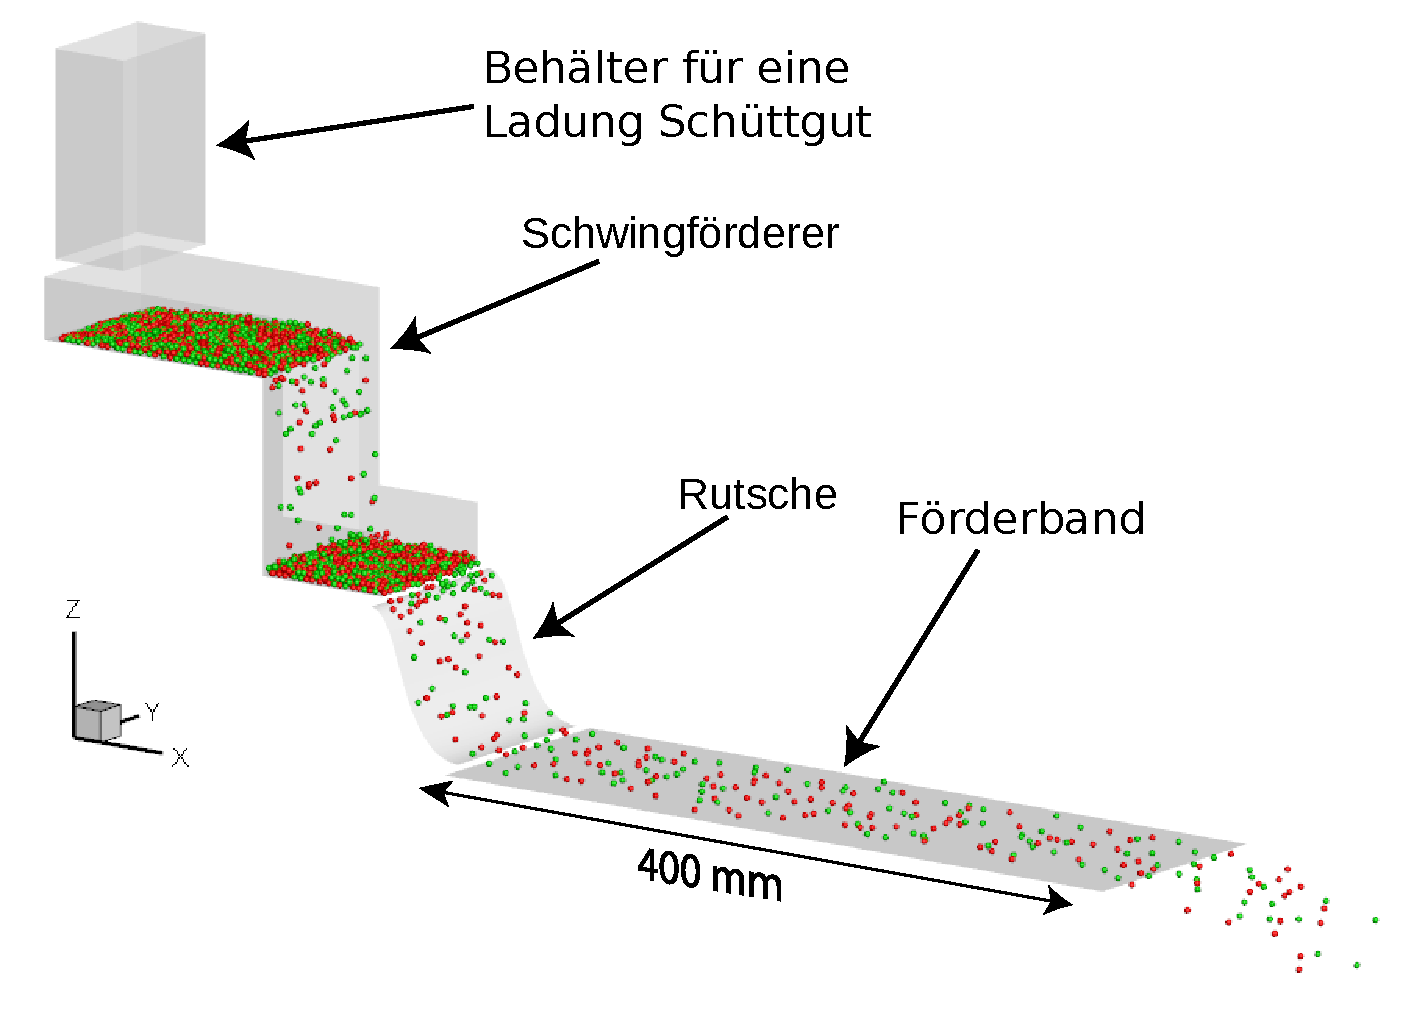
\includegraphics[width=\textwidth]{DEM-SimOverview}
	\caption{Visualisierung der DEM Simulation~\cite{Pfaff2018}}
	\label{fig:DEMSimulation}
\end{figure}


\section{Menge}

Insgesamt wurden 265451 Bilder aufgenommen.
177951 Bilder auf dem Förderband
87500 Bilder auf der Rutsche


Anzahl separate Tracks.
Anmerkung: Simulationsdaten sind die echte Wahrheit, während die werte von den Selbstgesammelten Daten hier 
auf die Korrektheit des Outputs vom Tracksort Algorithmus beruhen. 

Es wurden 
7538 Kugeln in 15 Batches,
7056 Pfefferkörner in 13 Batches,
17049 Zylinder in 11 Batches
und 8549 Weizenkörner in 13 Batches aufgenommen.
\todo[inline]{das in eine Schöne Tabelle stecken und erzählen}

\todo[inline]{Table mit Anzahl von Elementen in verschiedenen Batches}

\begin{figure}[h]
    \centering
    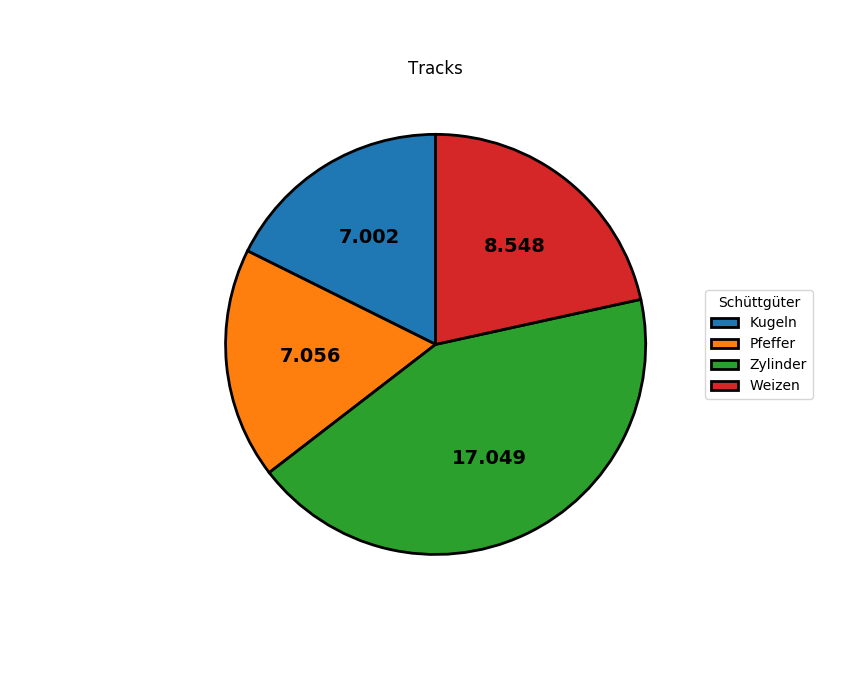
\includegraphics[width=\textwidth]{img/scaledPieChart-trimmed}
    \caption{Verteilung Schüttgut Elemente nach Sorte}
    \label{piechartSchuettgut}
\end{figure}


% Menge in gecleanten Daten:

% 7343 Kugeln
% 6824 Pfefferkörner
% 15760 Zylinder
% 8426 Weizenkörner


\section{Daten Postprocessing}

Cleanup : FilterTracksByAngle, FilterByVectorLengthChange \todo{Überlegen ob ich da so viel aufschreiben soll - 
minimaler unterschied nach Resegment (Bessere Tracksort zuordnung?)}

\color{blue}
\begin{itemize}
	\item Data Augmentation: Definition und Beschreibung
	\item bei Bildern normalerweise Rotieren, Translation, Ausschnitte...
	\item Hier: Spiegeln
	\item in einem Band - an der Mitte, nicht die Ränder mit nehmen - Kamera nicht perfekt zentriert
	\item Band zentrierung filter
	\item führt zu: Beinah verdoppelung der Feature-Label-paare fürs training.
\end{itemize}
\color{black}

Als Data Augmentation bezeichnet man Verfahren, die die eigenen Daten erweitern ohne zusätzliche Daten aufzunehmen.
Man generiert aus den bestehenden Daten zusätzliche, synthetische Daten, die dann im Trainingsset eingesetzt werden können.
Ausreichend viele Trainingsbeispiele zu haben ist notwendig um mit neuronalen Netzen eine gute Performance zu erzielen.
Die synthetischen Beispiele müssen jedoch plausibel sein, da sie sonst die Qualität der Ausgabe des Netzes negativ beeinträchtigen können.

Für Netze, die in der Bilderkennnung eingesetzt werden gibt es einige weit verbreitete Techniken,
zum Beispiel Rotation, Translation, Spiegeln und das Ausschneiden von Teilbildern.

Für den gegebenen Fall mit den Mittelpunkten von Schüttgut Partikeln als Features resultiert von diesen Techniken nur das Spiegeln in sinnvollen Daten.
gespiegelt wird an der Mittellinie entlang der Bewegungsrichtung.
Tracks, die [zu nah an den Rand kommen] werden ausgenommen, da zumindest bei den selbst aufgenommenen Daten, die Kamera nicht perfekt zentriert ist.

\begin{figure}[h]
	% \missingfigure{Visualisierung Dataaugmentation}
	\centering
	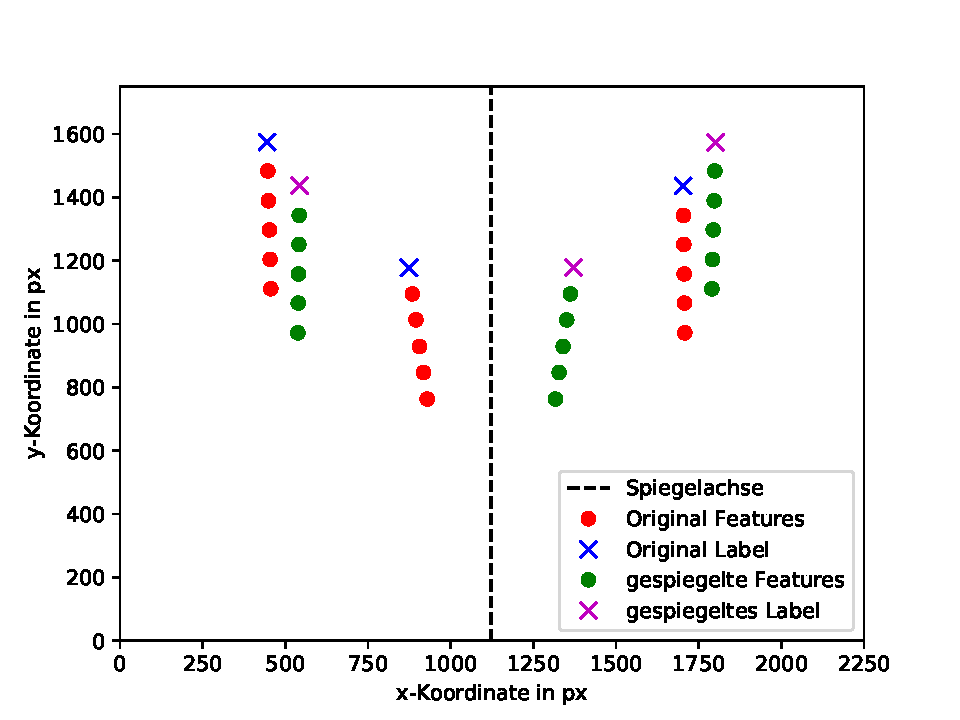
\includegraphics[width=\textwidth]{augmentationImage}
	\caption{Visualisierung Data Augmentation durch Spiegelung}
	% \todo{Quelle Bild!}
	\label{fig:dataAugm}
\end{figure}



\section{Trainingsbeispiele}

Train - Test - Validation - Split:
Train - test, 90\% zu 10\%.
Validation nur für die sets auf denen das Hyperparameter Tuning gemacht wurde
[ungefähres ]


Features:
NextStep einfach alle \(n\)--Tupel, die ein Track hergibt, sodass es noch ein Label geben würde
Separator: Muss unterschieden werden - Filtern oder nicht filtern, danach ob es das letzte mögliche Tupel vor der prediction Phase ist.
Mit filtern besseres ergebnis, aber auch deutlich weniger Trainingsbeispiele (Overfitting wird mehr zur Gefahr)
Ohne Filtern: Flexibler und mehr Trainingsbeispiele - man könnte im Nachhinen den PredictionCutOff verlegen 
und einfach das Netz weiter verwenden ohne neu zu trainieren.
Maybe ein Mittelding, das man nicht alle tupel nimmt aber auch nicht nur die letzten? Ausblick, zukunft



Labels:
Sehr straight forward für NextStep (Literally), einfach die nächste Zeile im Track jeweils für X und Y

für separator slightly more complicated: 
Element des Tracks vor und hinter der Separator position (entlang der Travel Achse)

Schnittpunkt geometrisch bestimmen.
Label für position ist die Position entlang der Achse orthogonal zur Bewegungsrichtung vom Schnittpunkt der Separatorlinie und 
der Strecke zwischen dem Element vor und dem element hinter. siehe \ref{fig:Schnittpunkt}




\todo{table of size of different data sets - number of pictures...}

Verhältnis: Anzahl Feature-Label-Paare für verschiedene Beispiele und verschiedene Settings
(FeatureSize, Filter Ja/Nein, Augmentation Ja/Nein) Als Tabelle?

OUTDATED:
Bei einer FeatureSize von 5 ergeben sich bei den Kugeln so 98.966 Feature-Label Paare.
Die Pfefferkörner haben dann 105.101 Feature-Label Paare,
bei den Zylindern kommt man auf 244.422 Feature-Label Paare
und bei den Weizenkörner 132.140 Feature-Label Paare.
